\chapter{Decision Trees}

Decision trees are another group of supervised learning algorithms.
They are used for both classification and regression problems.
Decision trees are easy to understand and interpret, and they are
very useful for exploratory data analysis. 
They are also the basis for more sophisticated methods we will introduce at the end of this chapter.
Similar to the KNN algorithm, decision trees are also non-parametric methods, which use the data 
as the model itself.
But different to the KNN algorithm, decision trees are non linear algorithms in the classical sense.
We will also see that there is a relation of decision trees to linear models.

\section{Classification Trees}
In this chapter and in the book we will only look into classification trees.
The regression trees are very similar, but we will not discuss them here.

Before we begin, we must introduce important concepts that construct decision trees.

A \textit{tree} is a hierarchical structure consisting of \textit{nodes} and \textit{edges}.
Nodes are connected by edges, and the edges are directed from the \textit{parent} node to the \textit{child} node.
For simplicity, we will only consider binary trees, where each node has at most two children.
Nodes without children are called \textit{leaves} or \textit{terminal nodes}, and nodes with children are called \textit{internal nodes} or \textit{decision nodes}.
The top node of a tree is called the \textit{root node}.
You can see a very simple example of a tree in Figure \ref{fig:tree_simple}.
\begin{figure}[ht]
  \centering
  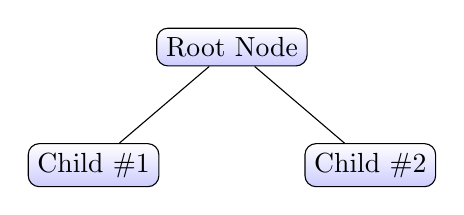
\begin{tikzpicture}[sibling distance=10em,
    every node/.style = {shape=rectangle, rounded corners,
      draw, align=center,
      top color=white, bottom color=blue!20}]]
    \node {Root Node}
      child { node {Child \#1} }
      child { node {Child \#2} };
  \end{tikzpicture}
  \caption{Simple decision tree.}
  \label{fig:tree_simple}
\end{figure}

\subsection{Motivational Examples}
Let us consider a simple example to motivate the idea of decision trees.
Imagine you want to plan a dinner party. And you need to decide whether you host
the party inside or outside. You have a lot of friends, and you want to invite as many as possible.

You come up with the decision tree shown in Figure \ref{fig:tree_dinner}.
\begin{figure}[ht]
  \centering
  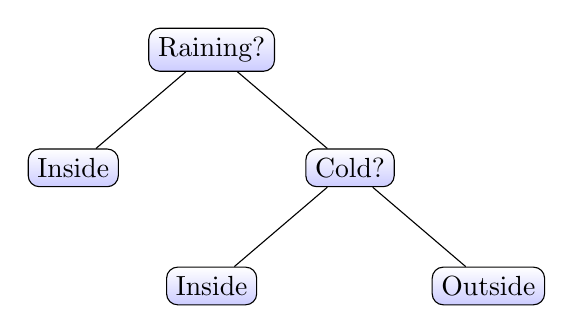
\begin{tikzpicture}[sibling distance=10em,
    every node/.style = {shape=rectangle, rounded corners,
      draw, align=center,
      top color=white, bottom color=blue!20}]]
    \node {Raining?}
      child { node {Inside} }
      child { node {Cold?}
        child { node {Inside} }
        child { node {Outside} }
      };
  \end{tikzpicture}
  \caption{Decision tree for planning a dinner party. Left nodes answer the short questions with \textit{yes}, right nodes with \textit{no}.}
  \label{fig:tree_dinner}
\end{figure}
From looking at this tree we can make two major observations.
First, the tree is a sequence of binary questions that we can answer with \textit{yes} or \textit{no}.
Second, the tree is a sequence of decisions that lead to a final decision.
We can also see that the tree is a sequence of \textit{if-then-else} statements.\\
If it is raining, we host the party inside, else we ask the next question.\newline
If it is cold, we host the party inside, else we host the party outside.

This sounds simple to implement, but how do we come up with these questions?
\subsection{Building a Decision Tree}
In a very simplistic way to build a decision tree, we need to follow the following three steps
\begin{enumerate}
  \item Split the data in "the best way possible"
  \item continue this process with every new left and right side, until satisfied
  \item create leaf nodes for final splits, assign label of majority of remaining samples to the leaf node
\end{enumerate}
But what does "the best way possible" mean? We will try to understand this based on the following example.
\subsection{Linearly Seperable Data}
Given the following linear seperable data $X$ and accomodating labels $y$, find the correct split to perform binary classification
\begin{align}
  X = \begin{bmatrix}
    0.3\\0.37
  \end{bmatrix},
  \begin{bmatrix}
    0\\1
  \end{bmatrix}
\end{align}
The solution to this is rather obvious
\begin{align}
f(x) = 
\left\{
\begin{matrix}
0 \text{ if } x \leq 0.3\\
1 \text{ if } x > 0.3
\end{matrix}
\right.
\end{align}
or as a decision tree (Figure \ref{fig:tree_linear_1}).
\begin{figure}[ht]
  \centering
  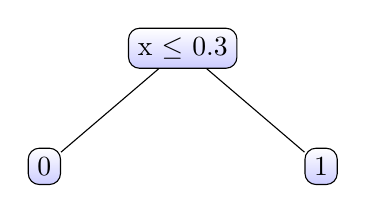
\begin{tikzpicture}[sibling distance=10em,
    every node/.style = {shape=rectangle, rounded corners,
      draw, align=center,
      top color=white, bottom color=blue!20}]]
    \node {x $\leq$ 0.3}
      child { node {0} }
      child { node {1} };
  \end{tikzpicture}
  \caption{Decision tree for very simplistic linear seperable data.}
  \label{fig:tree_linear_1}
\end{figure}

We can break down the decision process for the numerical value $x$ and selected threshold $0.3$ into two steps
\begin{enumerate}
  \item Select the best possible feature
  \subitem In this case, we only have one feature, so we do not need to select one
  \item Find the value in $x$ that separates the classes best
  \subitem In this case, we can see that the value $0.3$ is the only value available that represents the class $0$ and $0.37$ the only sample of class $1$
\end{enumerate}

With increasing amount of data points this process becomes increasingly hard to perform, manually.

Consider the following data
\begin{align}
X = \begin{pmatrix}
0.35, 0.6, 0.67, 0.8
\end{pmatrix}^T\\
y = \begin{pmatrix}
0, 0, 1, 1
\end{pmatrix}^T
\end{align}
The optimal solution is still very obvious
\begin{align}
f(x) = 
\left\{
\begin{matrix}
0 \text{ if } x \leq 0.6\\
1 \text{ if } x > 0.6
\end{matrix}
\right.
\end{align}
or as tree
\begin{figure}[ht]
  \centering
  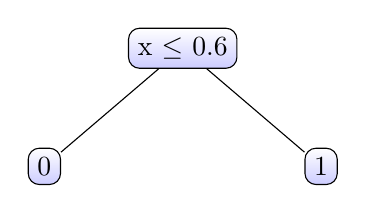
\begin{tikzpicture}[sibling distance=10em,
    every node/.style = {shape=rectangle, rounded corners,
      draw, align=center,
      top color=white, bottom color=blue!20}]]
    \node {x $\leq$ 0.6}
      child { node {0} }
      child { node {1} };
  \end{tikzpicture}
  \caption{Decision tree for more linear seperable data.}
  \label{fig:tree_linear_2}
\end{figure}

\subsection{Non-Linearly Seperable Data}
Given the following non-linear seperable data $X$ and accomodating labels $y$, find the correct split to perform binary classification
\begin{align}
X = \begin{pmatrix}
0.3, 0.1, 0.21, 0.35, 0.6, 0.67, 0.8, 0.786, 0.97
\end{pmatrix}^T\\
y = \begin{pmatrix}
0, 0, 1, 0, 1, 1, 0, 1, 0
\end{pmatrix}^T
\end{align}
In this example we can not simply split the data by briefly looking at it and visually recognize
the seperation. We need to find a way to split the data in a way that we can seperate the classes
as good as possible. For this we need to understand what a split actually is, how we can evaluate
the quality of a split and how we can find the best split. Additionally, when we have
multivariate data, we need to understand how we can select the best feature to split on.

\section{Information Gain}
The information gain $\text{Gain}$ tells us how much information we gain over $x$ while looking at $y$.
This metric can be used to evaluate the quality of a split. It measures the reduction
of an impurity metric in a splitted data set.
The information gain is defined as
\begin{align}
  \text{Gain}(S, V) = I(S) - \sum_{S_v\in V} \frac{|S_v|}{|S|}I(S_v)
\end{align}
with $V$ a set of splits out of $S$.  
For two splits
\begin{align}
\text{Gain}(S, V) = I(S) - \left(\frac{|S_1|}{|S|}I(S_1)+\frac{|S_2|}{|S|}I(S_2)\right)
\end{align}

\section{Impurity Metrics}
The impurity metric $I$ is a metric that measures the impurity of a data set.
The following metrics are calculated at the node level. The lower their value, the purer the observed data.
\subsection{Entropy}
The entropy is a measure of the uncertainty of a random variable and ranges from $0$ to $1$. It is defined as
\begin{align}
  I(S) = -\sum_{i=1}^n p_i \log_2 p_i
\end{align}
with $p_i$ the probability randomly selecting a sample of class $i$ out of the $k$ classes in $S$.

In Python, we can calculate the entropy as follows
\begin{lstlisting}[language=Python]
def entropy(s):
  counts = np.bincount(np.array(s, dtype=np.int64))
  percentages = counts / len(s)
  return -np.sum([
    pct*np.log2(pct)
    for pct in percentages
    if pct > 0
  ])
\end{lstlisting}

\subsection{Gini Impurity}
The Gini impurity is a measure of the probability of a random sample being classified incorrectly if it was randomly labeled according to the distribution of labels in the subset. Hence it combines the probability of randomly selecting an item $i$
\begin{align}
  p_i = \frac{|S_i|}{|S|}
\end{align}
with the probability of misclassifying an item $i$
\begin{align}
  \sum_{j\neq i} p_j = 1 - p_i = \frac{|S| - |S_i|}{|S|}
\end{align}
Thereby, the Gini impurity is defined as
\begin{align}
  I(S) = \sum_{i=1}^cp_i (1 - p_i) = \sum_{i=1}^c (p_i - p_i^2)\\
  = \underbrace{\sum_{i=1}^c p_i}_{:= 1} + \sum_{i=1}^c p_i^2 = 1 - \sum_{i=1}^c p_i^2
\end{align}

In Python, we can calculate the Gini impurity as follows
\begin{lstlisting}[language=Python]
def gini_impurity(s):
    counts = np.bincount(np.array(s, dtype=int))
    percentages = counts / len(s)
    return 1 - (percentages**2).sum()
\end{lstlisting}

Both metrics are very similar, but the Gini impurity is slightly faster to compute due to the lack of logarithm.
They also share some properties. A low impurity measure translates to a low likelihood of misclassification. A high value translates to a high likelihood of misclassification.

\subsection{Prediction Error}
Another metric is the prediction error. It is defined as
\begin{align}
  I(S) = 1 - \max_i p_i
\end{align}
and is essentially the inverse of the maximum probability of correctly classifying a sample for any given class in $S$.\\
This metric is not as useful as the other two to construct decision trees, but it is useful to evaluate the quality of a tree to optimize it.
One way of optimizing decision trees is to reduce their amount of decision nodes.
This can be done by pruning the tree. Pruning is the process of removing decision nodes from a tree.
We will discuss this in more detail shortly.

Implemented in Python, the prediction error looks like this
\begin{lstlisting}[language=Python]
def prediction_error(s):
    counts = np.bincount(np.array(s, dtype=int))
    percentages = counts / len(s)
    return 1 - np.max(percentages)
\end{lstlisting}

\subsection{Comparison of Impurity Metrics}
For comparison we will compute the impurity meytics for 101 different combinations of binary labels for 100 samples.

In Python, we could do something like this
\begin{lstlisting}[language=Python]
g = list(); e = list(); e2 = list(); err = list(); bins = list()
for i in range(101):
    values = [0] * (100 - i) + [1] * i
    g.append(gini_impurity(values))
    e.append(entropy(values))
    e2.append(np.array(entropy(values))/2.)
    err.append(error(values))
    bins.append(values)
\end{lstlisting}
and we can visualize these results with the following code
\begin{lstlisting}[language=Python]
import matplotlib.pyplot as plt

def draw_bins(bins, alpha=0.5):
  for idx, val in enumerate(bins):
    unique, counts = np.unique(val, return_counts=True)
    if idx == 0:
      counts = np.array([len(val), 0])
    elif idx == len(bins) - 1:
      counts = np.array([0, len(val)])
    plt.bar(
      [idx,idx+0.5],
      height=counts/len(val),
      width=0.5,
      color=['b', 'g'],
      label=['class 0', 'class 1'],
      alpha=alpha
    )
\end{lstlisting}
\begin{figure}[ht]
  \begin{minipage}{0.5\textwidth}
    \centering
    \includesvg[width=.95\textwidth]{images/DT_comparison_1.svg}
    \caption{Impurity metrics for 101 different combinations of binary labels for 100 samples.}
    \label{fig:impurity_metrics}
  \end{minipage}
  \begin{minipage}{0.5\textwidth}
    \centering
    \includesvg[width=.95\textwidth]{images/DT_comparison_2.svg}
    \caption{Rescaled impurity metrics for 101 different combinations of binary labels for 100 samples.}
    \label{fig:impurity_metrics_zoomed}
  \end{minipage}
\end{figure}
The entropy ranges from $0$ pure to $1$ impure, whereas the Gini impurity ranges from $0$ pure to $0.5$ impure as you can see in Figure \ref{fig:impurity_metrics}.
To visualize the relationship between the two metrics, we can rescale the entropy by dividing it by $0.5$. 
This allows us to see that the Gini impurity lies between the Entropy and the prediction error and is not a differently scaled Entropy (see Figure \ref{impurity_metrics_zoomed}).

Depending on the chosen metric the resulting trees can vary. Sometimes this makes a small impact,
sometimes a bigger one. Overall, Entropy and Gini impurity are implemented in many algorithms.
CART (Classification and Regression Trees) uses the Gini impurity, whereas ID3 (Iterative Dichotomiser 3) uses the Entropy.

Most of these implementations like C5 are highly optimized using methods like \textit{boosting}
 that improve the structure of the trees by selecting better splits.

\section{Disadvantages of Decision Trees}
The biggest and main disadvantage of decision trees is that deep trees are prone to overfitting the training data. On the other hand, shallow trees increase the risk of biased predictions.

One solution for this is called \textit{Random Forrest}. It is an ensemble method that combines multiple decision trees to reduce the risk of overfitting without sacrificing bias.
Random Forrests are more robust and generally better solvers than single decision trees.

You can find an implementation based on NumPy in the accomodating Jupyter notebook to this chapter.
